%!TEX program = xelatex
\documentclass[a4paper,UTF8]{article}
\usepackage[unicode=true,colorlinks,urlcolor=blue,linkcolor=blue,citecolor=red,bookmarksnumbered=true]{hyperref}
\usepackage{latexsym,amssymb,amsmath,amsbsy,amsopn,amstext,amsthm,amsxtra,color,multicol,bm,calc,ifpdf}
\usepackage{ctex}
\usepackage{graphicx}
\usepackage{diagbox}   % 绘制表格斜线
\usepackage{enumerate}
\usepackage[numbers,authoryear]{natbib}
\usepackage{fancyhdr}
\usepackage{subfig}
\usepackage{listings}
\usepackage{multirow}
\usepackage{makeidx}
\usepackage{xcolor} 
\usepackage{float}
\usepackage{geometry}
\geometry{a4paper,scale=0.7}
% \geometry{a4paper,left=2cm,right=2cm,top=1cm,bottom=1cm}

\graphicspath{{figures/}}  % 设置图片搜索路径

\newcommand\diff{\,{\mathrm d}}     % 定义微分 d
\newcommand{\p}[3]{\frac{\partial^{#1}#2}{\partial{#3}^{#1}}}  % 定义求偏导算子

\renewcommand\contentsname{Contents}
\renewcommand\refname{References}
\renewcommand\figurename{Figure}
\renewcommand\tablename{Table}


\begin{document}
\title{
	\includegraphics[width = 0.85\textwidth]{pku.pdf}\\
	\vspace{2em}
	\textbf{\huge{深度学习算法与应用期末作业报告}}\\
	\vspace{1em}
	\large{题目\ \underline{\makebox[26em]{基于图卷积神经网络的蛋白亚细胞定位预测}}}
}

\author{姓名\ \underline{\makebox[24em]{曹智杰,李响,郭宇航}}\\
	学号\ \underline{\makebox[24em]{1701110560,1701111447,1701110049}}\\
	学院\ \underline{\makebox[24em]{生命科学学院,前沿交叉学科研究院,数学科学学院}}\\
	专业\ \underline{\makebox[24em]{生物信息学,整合生命科学,统计学}}
}

\date{2018 年 8 月 30 日}


\maketitle
\thispagestyle{empty}

\newpage


\tableofcontents

\newpage

\section*{}
\begin{abstract}
	\quad 如何将图结构信息应用于图节点的分类问题一直是一个备受关注的问题。在本工作中,我们应用了2016年Kipf等人发展的图卷积神经网络(GCN)模型,利用蛋白质相互作用网络信息和基于卷积神经网络(CNN)模型提取的蛋白质序列特征进行蛋白质11种主要细胞亚定位进行预测,取得了比未利用蛋白质互作信息的模型和未使用CNN提取的特征的模型更好的预测功效,表明GCN模型在蛋白质细胞亚定位预测问题上具有的优越性。相关的数据集和代码见https://github.com/Jeff1995/pLocNet。
 \\
 
	\noindent{\heiti 关键字:} 图卷积神经网络;蛋白质细胞亚定位;分类问题.
\end{abstract}\thispagestyle{empty}
\newpage{}
\section{问题背景}
\subsection{图卷积模型}

现实世界中有许多重要的数据集以图或网络的形式出现:如社交网络,知识图谱,蛋白质交互网络,万维网等等。然而,迄今为止人们也很少关注神经网络模型对这种结构化数据集的推广应用。\\

如何完善地推广神经网络模型(如RNN或CNN)来处理任意结构化图形数据是一个具有挑战性的问题。最近的一些工作介绍了特定问题的网络架构(Duvenaud et al., NIPS 2015; Li et al., ICLR 2016; Jain et al., CVPR 2016),其他人则利用谱图理论中的图形卷积(Bruna et al., ICLR 2014; Henaff et al., 2015)来定义用于多层神经网络模型的参数化滤波器,类似于我们所熟知和喜爱的“经典”CNN。\\

最近的工作重点是跨越快速启发式的算法和高昂的计算复杂度之间的鸿沟。Defferrard et al. (NIPS 2016)使用切比雪夫多项式在谱域中近似平滑滤波器,其中所述的自由参数在类似神经网络的模型中学习。它们在常规数据集(如MNIST)上取得令人信服的结果,与简单的2D-CNN模型非常接近。Kipf&Welling等人采用了一种类似的方法(ICLR 2017),从谱图卷积的框架开始,然后引入简化近似,从而兼得显著加快训练时间和提高预测准确性这两个优点,最后在许多基准图数据集上达到最先进的分类结果。\\

目前,大多数图形神经网络模型具有一些共同的通用架构。 Kipf等人将这些模型称为图形卷积网络(GCN);之所以被称为卷积,是因为滤波器参数通常在图中的所有位置共享(或其子集,如Duvenaud et al., NIPS 2015)。\\

对于这些模型,目标是在图形$G=(V,E)$上学习信号/特征的函数;输入如下:
\begin{itemize}
	\item 每个节点$i$的特征描述$x_i$,总结在一个$N×D$的特征矩阵$X$中($N$:节点数,$D$:输入特征数);
	\item 反映节点之间关系的图结构的代表性描述,通常以邻接矩阵$A$的形式;
\end{itemize}

输出是描述节点特征的$N×F$矩阵$Z$,其中$F$是每个节点的输出特征数)。\\

Kipf等人将每个神经网络层写为非线性函数:\\
$$H^{(l+1)}= f(H^{(l)},A)$$
其中 $H^{(0)}= X$且$H^{(l)}= Z$,$L$为层数。具体模型的区别仅在于如何选择和参数化$f(\cdot,\cdot)$。\\

Kipf等人使用了以下的隐含层迭代规则:\\
$$f(H^{(l)},A) = \sigma(AH^{(l)}W^{(l)})$$
其中$W^{(l)}$是第$l$个神经网络层的权重矩阵,$\sigma(\cdot)$是类似ReLU的非线性激活函数。尽管它很简单,但这个模型已经非常强大了,在文献引用网络和知识网络的数据集中表现出了良好的预测性能。\\

这个简单的模型存在两个局限:首先,每步迭代中乘以A意味着,对于每个节点,我们将所有相邻节点的所有特征相加而没有节点本身。通过在图中添加自环,即将单位矩阵添加到A可以解决这个问题。\\

第二个主要限制是A通常不归一化,因此与A的乘法将完全改变特征向量的数量级(可以通过查看A的特征值来理解)。归一化A使得所有行总和为1,即$D^{-1}A$,其中D是对角节点度矩阵,从而摆脱了这个问题。与$D^{-1}$相乘意味着取相邻节点特征的平均值。实际上,当使用对称归一化时,算法变得更有趣,即$\widetilde{A}={D}^{-\frac{1}{2}} {A} {D}^{-\frac{1}{2}} $。这两个技巧的结合即可得出Kipf&Welling(ICLR 2017)中的传播规则:

\[ H^{(l+1)} = f(H^{(l)},A) = \sigma \left( \hat{D}^{-\frac{1}{2}} \hat{A} \hat{D}^{-\frac{1}{2}} H^{(l)}W^{(l)}\right)\]
其中$\hat{A}= A + I$,$I$是单位矩阵,$\hat{D}$是对角节点度矩阵。

这个式子的意义显而易见:每一步隐含层的取值都是上一步相邻节点的平均值再经过激活函数变换后的结果。为了进一步说明这个表达式的来源和优点,以下将进一步阐述它的理论动机。\\

考虑多层图形卷积网络(GCN)的分层传播规则,我们将要证明这种传播规则的形式可以通过图上的局部光谱滤波器的一阶近似来启发得到(Hammond et al., 2011; Defferrard et al., 2016)。\\

符号说明:图的(归一化)拉普拉斯矩阵$L$可以很容易从对称归一化图邻接矩阵$\widetilde{A}$计算出来:$L = I_N-\widetilde{A} = I_N-{D}^{-\frac{1}{2}} {A} {D}^{-\frac{1}{2}} = U \Lambda U'$。值得一提的是这两个矩阵具有特殊的性质:$\widetilde{A}$的最大特征值是1,最小特征值不小于-1;从而$L$的特征值也都介于0和2之间。\\

图傅里叶变换被定义为图信号$X$(即每个节点的特征向量)与图的拉普拉斯矩阵$L$的特征向量矩阵$U$的乘法,即$U'x$。频谱图卷积被定义为信号与图的傅立叶空间中的滤波器的乘法,滤波器以$g_\theta=diag(\theta)$表示,$\theta$是参数。于是有频谱图卷积表达式:
$$g_\theta \ast x = U g_\theta U' x$$
可以看出,上式的计算复杂度是比较大的,因为与特征向量矩阵$U$的乘法是$O(N^2)$的。 此外,首先计算$L$的特征分解对于大的图结构来说可能是非常高昂的。为了避免这个问题,Hammond et al. (2011) 提出)$g_{\theta}(\Lambda)$可以通过Chebyshev多项式$T_k(x)$直到K阶的截断展开很好地近似:
$$g_{\theta'}(\Lambda)\approx\sum\limits_{k=0}^K \theta'_k T_k(\widetilde{\Lambda})$$
重新调整的$\widetilde{\Lambda}=\frac{2}{\lambda_{max}}\Lambda-I_N$。$\lambda_{max}$表示L的最大特征值,一般近似取做2,$\theta$是切比雪夫多项式的系数,于是我们得到:
$$g_\theta' \ast x \approx \sum\limits_{k=0}^K \theta'_k T_k(\widetilde{L})x $$
$\widetilde{L}=\frac{2}{\lambda_{max}}L-I_N$,
这个表达式的计算复杂度是$O(\vert E \vert)$即与图的边数为线性关系。\\

现在,假设我们将逐层卷积运算限制为$K = 1$,得到了GCN的这种简化线性公式:
$$g_\theta \ast x \approx \theta'_0x + \theta'_1(L-I_N)x=\theta'_0x-\theta'_1{D}^{-\frac{1}{2}} {A} {D}^{-\frac{1}{2}} x$$
有两个自由参数,可以在整个图表上共享。在实践中,不妨进一步限制参数的数量可能是有益的,以解决过度拟合并最小化每层的操作(例如矩阵乘法)的数量。 这给我们留下了以下表达式:
$$g_\theta \ast x \approx \theta \left(I_N+{D}^{-\frac{1}{2}} {A} {D}^{-\frac{1}{2}} \right)x$$
使用单个参数$\theta=\theta_0=-\theta_1$。 注意,$I_N+{D}^{-\frac{1}{2}} {A} {D}^{-\frac{1}{2}}$具有特征值
范围[0,2]。 因此,当在深度神经网络模型中使用时,重复应用该算子可能导致数值不稳定性和梯度爆炸/消失的情况。 为了缓解这种问题,我们引入以下重整化技巧:$I_N+{D}^{-\frac{1}{2}} {A} {D}^{-\frac{1}{2}} \rightarrow \hat{D}^{-\frac{1}{2}} \hat{A} \hat{D}^{-\frac{1}{2}}$, 其中$\hat{A}= A + I_N$\\

我们可以将该定义推广到具有$C$个输入通道的信号,$X$为$N×C$维矩阵和F维的过滤器输出如下:
$$Z = \hat{D}^{-\frac{1}{2}} \hat{A} \hat{D}^{-\frac{1}{2}} X \Theta $$
其中$\Theta $为$C×F$维,现在作为滤波器参数矩阵,$Z$为$N×F$维是卷积信号矩阵。该滤波操作具有计算复杂度$O(\vert E \vert FC)$,因为关于$X$的矩阵乘法可以有效地实现为密集矩阵与稀疏矩阵的乘积。从而我们得到了一开始介绍的图卷积多层传播表达式。

\subsection{蛋白质亚细胞定位}

蛋白质亚细胞定位预测是一类重要的生物信息学问题。相关的预测工具通常以蛋白质本身的氨基酸序列信息为输入,输出预测的蛋白质细胞亚定位。它可以提供蛋白质功能和基因注释的信息,辅助药物靶点的识别。
<<<<<<< HEAD
现有的蛋白质亚细胞定位预测工具通常是从蛋白质的氨基酸序列中提取出一些特征,将序列转化为数值向量,再用机器学习模型进行预测。如目前最广泛使用的适用于真核生物蛋白质的WoLF PSORT软件,将蛋白质的氨基酸组成作为特征,以k-nearest neighbor算法给出与输入蛋白最相似的32个蛋白质的细胞亚定位。(Horton et al., 2007)我们认为,现有的预测工具还具有一定的提升空间。首先,提取的序列特征未必能充分反映蛋白质与训练任务相关的性质。其次,目前的预测都仅仅使用了蛋白质本身的信息,而没有考虑到蛋白质间的相互作用。考虑到蛋白质发生相互作用必须在空间上接近,蛋白质的相互作用信息很有可能可以提高亚细胞定位的预测准确度。因此,我们希望用神经网络将蛋白质序列embedding为数值向量,与蛋白质的相互作用信息结合,建立图卷积神经网络模型来进行蛋白质亚细胞定位的预测,以期能达到更好的预测功效。\\
=======
现有的蛋白质亚细胞定位预测工具通常是从蛋白质的氨基酸序列中提取出一些特征,将序列转化为数值向量,再用机器学习模型进行预测。如目前最广泛使用的适用于真核生物蛋白质的WoLF PSORT软件,将蛋白质的氨基酸组成作为特征,以k-nearest neighbor算法给出与输入蛋白最相似的32个蛋白质的细胞亚定位。(这里要插入一篇引用)我们认为,现有的预测工具还具有一定的提升空间。首先,提取的序列特征未必能充分反映蛋白质与训练任务相关的性质。其次,目前的预测都仅仅使用了蛋白质本身的信息,而没有考虑到蛋白质间的相互作用。考虑到蛋白质发生相互作用必须在空间上接近,蛋白质的相互作用信息很有可能可以提高亚细胞定位的预测准确度。因此,我们希望用神经网络将蛋白质序列embedding为数值向量,与蛋白质的相互作用信息结合,建立图卷积神经网络模型来进行蛋白质亚细胞定位的预测,以期能达到更好的预测功效。
(TODO: 是不是要加一下什么是蛋白,蛋白由20种氨基酸连接组成啥的,还有什么是亚细胞定位,序列与亚细胞定位的关系(motif,NLS, NES……)?)


>>>>>>> 2883f63780276cfec90320e013c6e2a7bd499165

\section{数据收集与预处理}

蛋白质互作网络数据来自STRING数据库,我们从人类蛋白的相互作用中筛选了作用模式为物理相互作用(physical)的蛋白对,用于后续模型训练。

蛋白亚细胞的定位和氨基酸序列数据来自UniProtKB/Swiss-Prot数据库:
其中,对于亚细胞定位注释,我们只保留存在文献支持的条目,经过滤后的定位注释有213种,大部分定位对应的蛋白都非常少(TODO: figure),我们只取蛋白数最多的11种亚细胞定位,包括细胞核(Nucleus),细胞质(Cytoplasm),细胞膜(Cell membrane),膜(Membrane),外泌(Secreted),细胞骨架(Cytoskeleton),细胞凸起(Cell projection),内质网膜(Endoplasmic reticulum membrane),细胞连接(Cell junction),线粒体(Mitochondrion)和高尔基体(Golgi apparatus);需要说明的是,这些亚细胞定位并不是互斥的,同一个蛋白可能会在多个位置出现并发挥功能。

\begin{figure}[H]
	\centering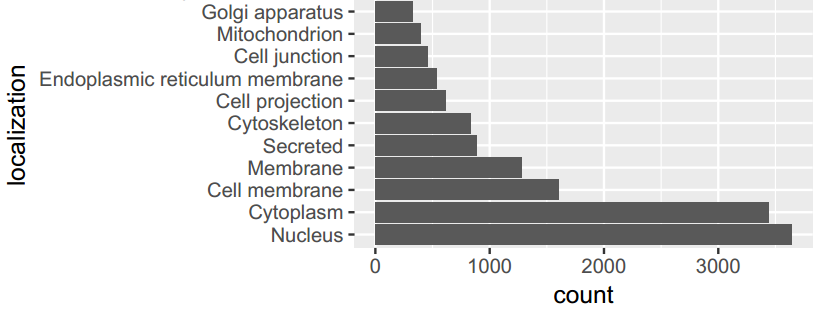
\includegraphics[scale=0.7]{../data/summary/loc.png}
\end{figure}
Figure 1.各亚定位的蛋白质数量分布。

对于氨基酸序列,我们丢掉了含有特殊氨基酸(硒半胱氨酸,Selenocysteine, U)的序列,所有序列只包含20种基本氨基酸;此外,相似序列在训练集和测试集中分别出现可能导致模型的预测性能被高估,因此我们使用cd-hit工具对序列进行了聚类,相似度高于90\%的序列作为一个类,只取其中一条序列作为代表,保证剩下的序列两两之间相似性低于90\%;最后,为了加快计算速度,我们只保留长度小于2000氨基酸的序列。
经过上述筛选之后,同时满足亚细胞定位和序列过滤条件,且在STRING蛋白互作网络中的担保共有7591条,构成模型评估的核心数据集。

\begin{figure}[H]
	\centering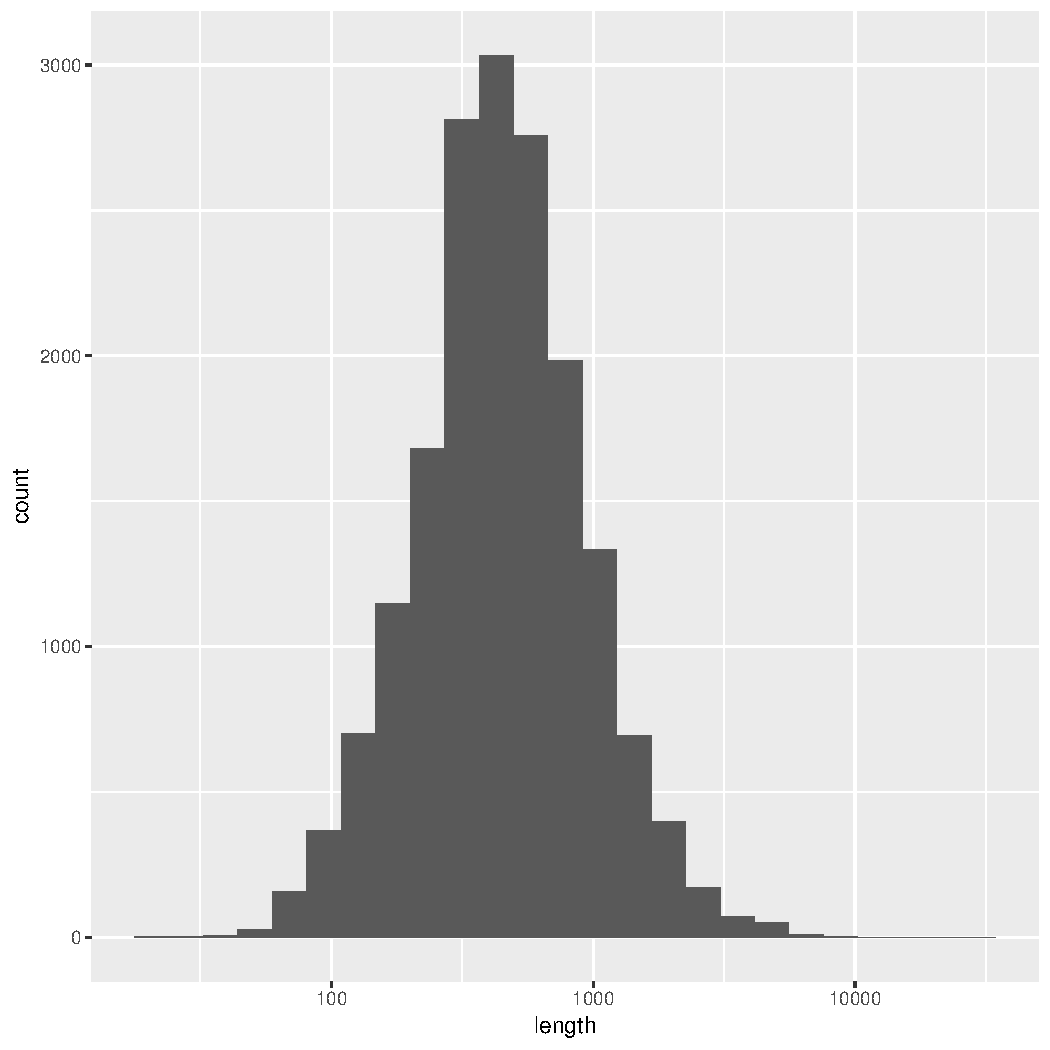
\includegraphics[scale=0.5]{../data/summary/seqlen.pdf}
\end{figure}
Figure 2.核心数据集蛋白质长度分布。

\section{模型构建}

\subsection{特征提取}

蛋白的亚细胞定位与其氨基酸序列有关,因此我们首先从氨基酸序列抽取可用的数据特征,一种传统特征提取方式是kmer频率,即根据蛋白质的氨基酸序列中所有长度为$k$的子片段出现的频率来作为该蛋白质的特征。氨基酸种类为20种,所以特征的维数为$20^k$,这里我们选取$k=3$,得到8000维的稀疏特征。\\

参考现有基于CNN的生物序列预测模型 (Alipanahi, B. et al., 2015; Zhou, J. $\&$ Troyanskaya, O.G., 2015),我们也尝试使用CNN来学习氨基酸序列中的motif,首先,每种氨基酸被编码成20维的one-hot向量(第$i$维为1代表这是第$i$种氨基酸),在此基础上,长度为$L$的蛋白(由$L$个氨基酸组成),可以表示成$L\times 20$的矩阵,类比图像数据相当于蛋白是有20个通道的一维“图像”;由于计算效率的原因,CNN一般要求输入具有相同的大小,而蛋白序列的长度是不确定的,因此我们以数据集中最长的蛋白为标准(长度<2000,见“数据收集与预处理”),在其他蛋白末尾补零,得到相同长度作为卷积输入,进行"valid"模式的卷积,并使用ReLU激活函数,只输出正值;在池化层,再按照序列长度屏蔽补零位置的信号(主要屏蔽补零边界上的信号),池化策略方面,我们使用全局最大和全局求和的折中,取$k$个最大值求和作为输出,这样使得池化输出不会受到蛋白长度的影响,同时又能反映相同序列motif多次出现的剂量效应。\\

我们尝试了两种基于CNN的蛋白序列特征提取方法,第一种是在训练集上进行有监督学习,第二种是在更大的无标签数据集上进行无监督学习;有监督学习比较常规,在池化层后面使用全连接层进行亚细胞定位预测,然后将倒数第二个全连接层的输出作为提取到的序列特征;无监督学习策略类似于噪音对比估计(noise contrastive estimation),具体做法是按照数据集中20种氨基酸的出现频率,随机生成氨基酸序列,随机序列的长度和真实序列一一对应,然后让CNN学习区分真实的蛋白序列和随机序列,这样我们期望CNN的卷积层能抓取到只有真实蛋白中高频出现的序列motif,可能与蛋白的生物学功能有关,其中就包括亚细胞定位,为了抓取尽可能多的motif,我们使用了较多卷积核,这样CNN学到的卷积核之间可能存在相关性,因此我们在CNN训练完成之后再使用一个变分自编码器VAE (Kingma, D.P. $\&$ Welling, M., 2013. Auto-Encoding Variational Bayes. arXiv.org, stat.ML.) 去拟合CNN池化层的输出,将VAE的隐变量作为最终序列特征,期望能得到信息更紧密的序列表示,具体来说,我们使用Gamma分布作为生成分布,模型的损失函数如下:

<<<<<<< HEAD
=======
\section{方法}

\subsection{数据收集与预处理}

蛋白质互作网络数据来自STRING数据库,我们从人类蛋白的相互作用中筛选了作用模式为物理相互作用(physical)的蛋白对,用于后续模型训练。
蛋白亚细胞的定位和氨基酸序列数据来自UniProtKB/Swiss-Prot数据库:
其中,对于亚细胞定位注释,我们只保留存在文献支持的条目,经过滤后的定位注释有213种,大部分定位对应的蛋白都非常少(TODO: figure),我们只取蛋白数最多的11种亚细胞定位,包括细胞核(Nucleus),细胞质(Cytoplasm),细胞膜(Cell membrane),膜(Membrane),外泌(Secreted),细胞骨架(Cytoskeleton),细胞凸起(Cell projection),内质网膜(Endoplasmic reticulum membrane),细胞连接(Cell junction),线粒体(Mitochondrion)和高尔基体(Golgi apparatus);需要说明的是,这些亚细胞定位并不是互斥的,同一个蛋白可能会在多个位置出现并发挥功能;
对于氨基酸序列,我们丢掉了含有特殊氨基酸(硒半胱氨酸,Selenocysteine, U)的序列,所有序列只包含20种基本氨基酸;此外,相似序列在训练集和测试集中分别出现可能导致模型的预测性能被高估,因此我们使用cd-hit工具对序列进行了聚类,相似度高于90\%的序列作为一个类,只取其中一条序列作为代表,保证剩下的序列两两之间相似性低于90\%;最后,为了加快计算速度,我们只保留长度小于2000氨基酸的序列(TODO: figure);
经过上述筛选之后,同时满足亚细胞定位和序列过滤条件,且在STRING蛋白互作网络中的蛋白共有7591条,构成模型评估的核心数据集。

\subsection{模型构建}

蛋白的亚细胞定位与其氨基酸序列有关,因此我们首先从氨基酸序列抽取可用的数据特征,一种传统特征提取方式是kmer频率(TODO: lix?);
参考现有基于CNN的生物序列预测模型 (Alipanahi, B. et al., 2015. Predicting the sequence specificities of DNA- and RNA-binding proteins by deep learning. Nature Biotechnology, 33(8), pp.831–838. Zhou, J. & Troyanskaya, O.G., 2015. Predicting effects of noncoding variants with deep learning-based sequence model. Nature Methods, 12(10), pp.931–934.),我们也尝试使用CNN来学习氨基酸序列中的motif,首先,每种氨基酸被编码成20维的one-hot向量(第i维为1代表这是第i种氨基酸),在此基础上,长度为L的蛋白(由L个氨基酸组成),可以表示成L*20的矩阵,类比图像数据相当于蛋白是有20个通道的一维“图像”;由于计算效率的原因,CNN一般要求输入具有相同的大小,而蛋白序列的长度是不确定的,因此我们以数据集中最长的蛋白为标准(长度<2000,见“数据收集与预处理”),在其他蛋白末尾补零,得到相同长度作为卷积输入,进行"valid"模式的卷积,并使用ReLU激活函数,只输出正值;在池化层,再按照序列长度屏蔽补零位置的信号(主要屏蔽补零边界上的信号),池化策略方面,我们使用全局最大和全局求和的折中,取k个最大值求和作为输出,这样使得池化输出不会受到蛋白长度的影响,同时又能反映相同序列motif多次出现的剂量效应。
我们尝试了两种基于CNN的蛋白序列特征提取方法,第一种是在训练集上进行有监督学习,第二种是在更大的无标签数据集上进行无监督学习;有监督学习比较常规,在池化层后面使用全连接层进行亚细胞定位预测,然后将倒数第二个全连接层的输出作为提取到的序列特征;无监督学习策略类似于噪音对比估计(noise contrastive estimation),具体做法是按照数据集中20种氨基酸的出现频率,随机生成氨基酸序列,随机序列的长度和真实序列一一对应,然后让CNN学习区分真实的蛋白序列和随机序列,这样我们期望CNN的卷积层能抓取到只有真实蛋白中高频出现的序列motif,可能与蛋白的生物学功能有关,其中就包括亚细胞定位,为了抓取尽可能多的motif,我们使用了较多卷积核,这样CNN学到的卷积核之间可能存在相关性,因此我们在CNN训练完成之后再使用一个变分自编码器VAE (Kingma, D.P. & Welling, M., 2013. Auto-Encoding Variational Bayes. arXiv.org, stat.ML.) 去拟合CNN池化层的输出,将VAE的隐变量作为最终序列特征,期望能得到信息更紧密的序列表示,具体来说,我们使用Gamma分布作为生成分布,模型的损失函数如下:
>>>>>>> 2883f63780276cfec90320e013c6e2a7bd499165
$$-\mathcal L(\theta, \phi) = \mathbb E_{z \sim q(z|x;\phi)} [\log p(x|z;\theta)] - KL(q(z|x;\phi) \parallel p(z))$$
其中,
$$p(z)=\mathcal N(0, I)$$
$$q(z|x;\phi)=\mathcal N(\mu_x, diag(\sigma_x^2))$$
$$KL(q(z|x;\phi) \parallel p(z)) = \frac 1 2 \sum_i (\mu_{i,x}^2 + \sigma_{i,x}^2 - \log \sigma_{i,x}^2 - 1)$$
$$\log p(x|z;\theta)=\alpha_z \cdot\ log \beta - \log \Gamma(\alpha_z) + (\alpha_z - 1) \cdot \log x - \beta \cdot x$$
后验分布的$\mu_x$, $\sigma_x^2$由$\theta$参数化的编码器网络实现,生成分布的$\alpha_z$由$\phi$参数化的解码器网络实现,$\beta$固定为定值,对$q(z|x;\phi)$的期望用reparameterization trick来计算;
为了公平,有监督和无监督序列特征都设定为100维。
<<<<<<< HEAD
=======

在上面得到的数据特征基础上,我们分别用全连接层和图卷积层构建预测网络,最终输出$p \in \mathbb R^J$各类别为阳性的概率,这里各类别没有互斥性,有监督损失函数使用的是$J$个二分类交叉熵的和:
$$\mathcal L(\theta) = \sum_i^N w_i \sum_j^{J} y_j\cdot \log p_j + (1-y_j)\cdot \log (1-p_j) $$
其中$w_i$是样本权重,为了平衡不同类别的样本,我们按照训练集中阳性和阴性的比例来给两种样本分别加权:
$$w_i=y_i \cdot (\frac N^++N^- 2N^+) + (1-y_i) \cdot (\frac N^++N^- 2N^-)$$

最后,我们使用5折交叉验证来进行模型评估,对于需要验证集的模型,从训练集中再随机抽取10\%作为验证集。

此外,为了评估蛋白质相互作用信息与亚细胞定位的关系,我们建立了一个不需要任何特征,仅依赖于蛋白质相互作用信息的预测模型,称之为GN(graph-neighbor)模型。对训练集或测试集中的任一蛋白质,我们根据训练集中与它有相互作用的蛋白质中具有某定位的蛋白质所占的比例来作为它具有该定位的概率,如果该蛋白质在训练集中没有邻居,则以整个训练集中具有该定位的蛋白质所占的比例作为其具有该定位的概率。

>>>>>>> 2883f63780276cfec90320e013c6e2a7bd499165

\subsection{模型训练}

<<<<<<< HEAD
在上面得到的数据特征基础上,我们分别用全连接层和图卷积层构建预测网络,最终输出$p \in \mathbb R^J$各类别为阳性的概率,这里各类别没有互斥性,有监督损失函数使用的是$J$个二分类交叉熵的和:
$$\mathcal L(\theta) = \frac{1}{N} \sum_{i=1}^N \sum_{j=1}^{J} w_j^{(i)} [y_j^{(i)}\cdot \log p_j^{(i)} + (1-y_j^{(i)})\cdot \log (1-p_j^{(i)})] $$
其中$w_j^{(i)}$是样本权重,为了平衡不同类别的样本,我们按照训练集中阳性和阴性的比例来给两种样本分别加权:
$$w_j^{(i)}=y_j^{(i)} \cdot (\frac {N_j^+ + N_j^-} {2N_j^+}) + (1-y_j^{(i)}) \cdot (\frac {N_j^+ +N_j^-} {2N_j^-})$$
=======
采用 Single-Index 模型较GLM相比已经有了很大的进步,我们继续尝试一些机器学习的方法对数据进行建模。
>>>>>>> 2883f63780276cfec90320e013c6e2a7bd499165

最后,我们使用5折交叉验证来进行模型评估,对于需要验证集的模型,从训练集中再随机抽取10\%作为验证集。\\

此外,为了评估蛋白质相互作用信息与亚细胞定位的关系,我们建立了一个不需要任何特征,仅依赖于蛋白质相互作用信息的预测模型,称之为GN(graph-neighbor)模型。对训练集或测试集中的任一蛋白质,我们根据训练集中与它有相互作用的蛋白质中具有某定位的蛋白质所占的比例来作为它具有该定位的概率,如果该蛋白质在训练集中没有邻居,则以整个训练集中具有该定位的蛋白质所占的比例作为其具有该定位的概率。

\section{实验结果与讨论}

各模型在11个细胞亚定位中的5折交叉验证AUC值如图3所示。可以看出,在所有细胞亚定位中,使用蛋白质互作信息的GCN模型的表现普遍高于未使用互作信息的神经网络模型。在所有模型中,基于有监督学习的CNN得到的特征进行训练的GCN模型具有最佳的预测功效。有监督学习的CNN得到的特征要优于使用VAE得到的特征,二者都优于3mer频率的特征。考虑到有监督学习更容易提取与任务相关联的特征,基于3mer频率的特征无法捕捉蛋白质的氨基酸序列中的长程相互作用信息,这一结果是符合我们的预期的。

\begin{figure}[H]
	\centering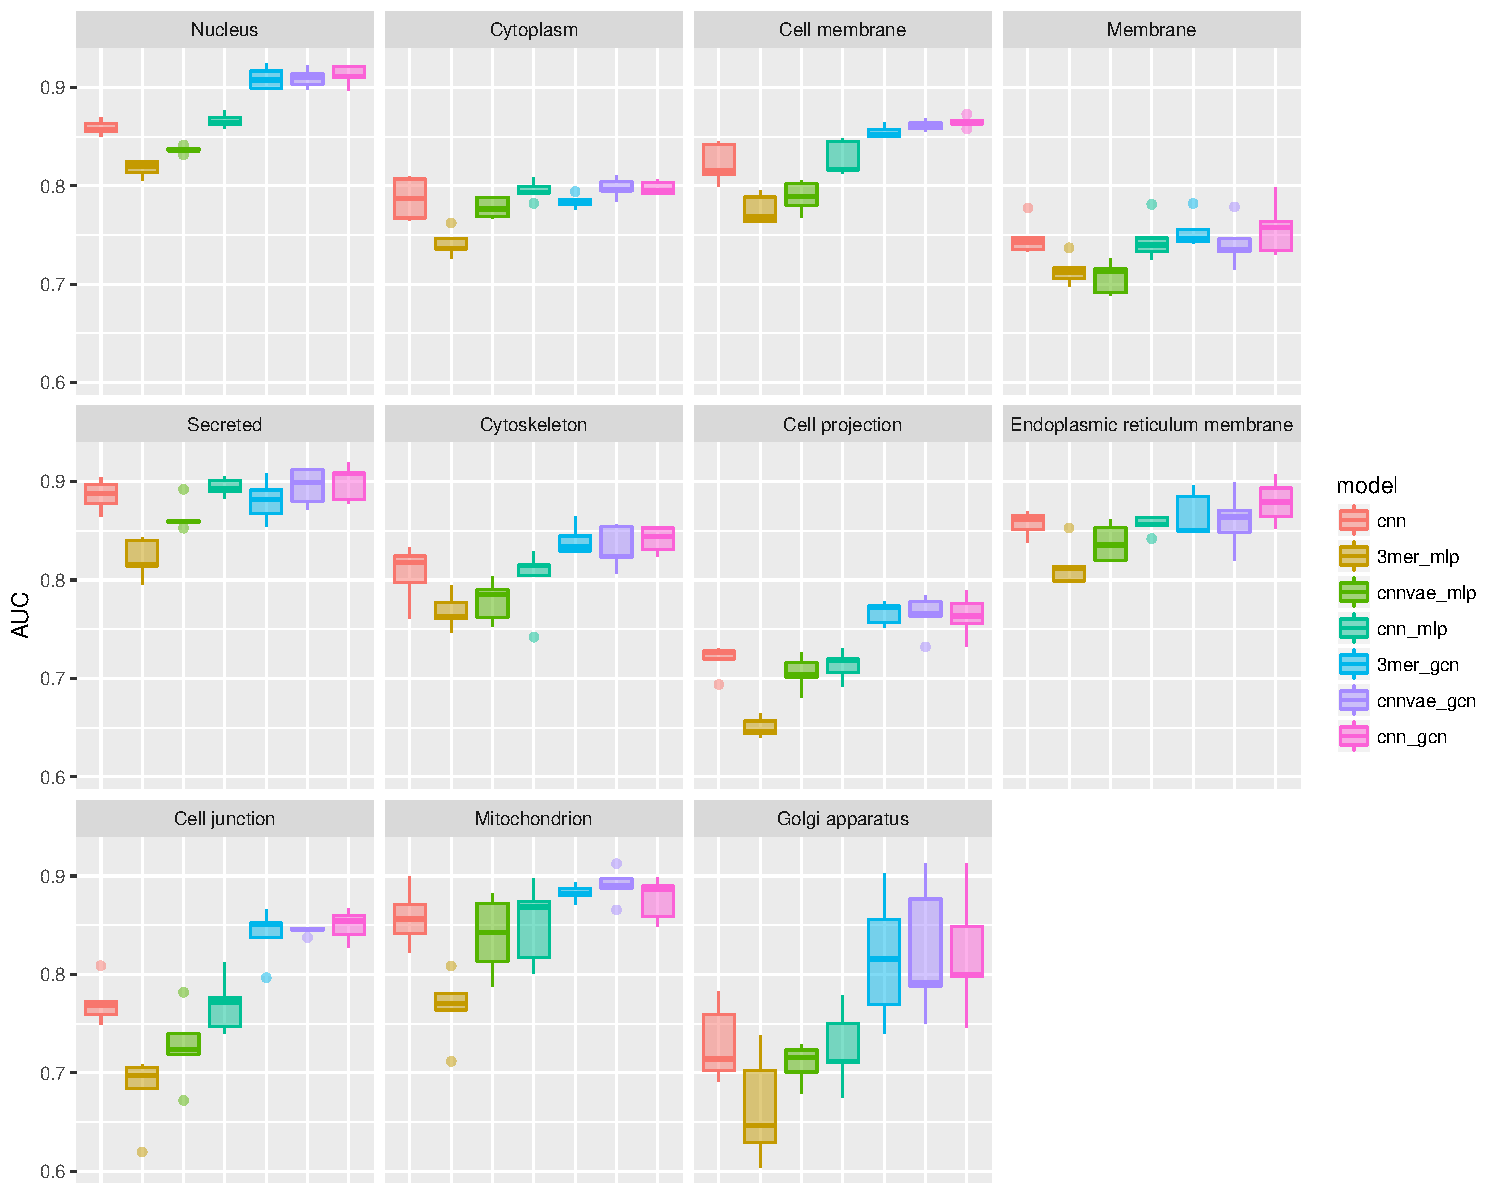
\includegraphics[scale=0.7]{../result/test_performance_AUC.pdf}
\end{figure}
Figure 3. 各模型在11种细胞亚定位上的验证AUC分布。\\

一个值得注意的现象是,仅依赖蛋白质互作信息的GN模型对于某些定位表现出较好的预测功效(如Nucleus,Cell projection,Golgi apparatus等),而对于另一些定位预测功效较差(如Membrane,Secreted,Endoplasmic reticulum membrane)。我们发现,预测功效较好的多是基质区域,而预测功效较差的则是膜结构和分泌型蛋白。我们认为这种差异来自于不同定位的蛋白相互作用的对象不同。在核内或细胞器基质的蛋白更多地与同一基质内的蛋白发生相互作用以发挥功能,而膜蛋白与胞质内蛋白或其它蛋白的分泌蛋白发生相互作用的比例更高。尽管如此,整合了蛋白质序列特征和互作信息的GCN模型依然可以表现出比仅使用序列特征的神经网络模型更佳的预测功效。我们认为,尽管蛋白质的相互作用并不等价于它们的共定位,但互作信息依然蕴含了与蛋白质身份和亚定位有关的序列信息。我们推测GCN模型通过将关联的隐含层输出进行线性组合,强化了这一部分特征的权重,从而提升了模型的预测功效。这与Kipf在他们的工作中所提出的观念相吻合,即GCN模型并不需要图中相邻节点具有相似的性质这一强假设。

\section{总结}

<<<<<<< HEAD
我们使用了Kipf等人发展的GCN模型,结合蛋白质互作网络与基于CNN有监督学习提取的蛋白质序列特征,在蛋白质的11种主要细胞亚定位的预测问题中取得了较好的预测功效。通过与仅基于蛋白质互作网络的GN模型进行比较,表明GCN不需要关联节点之间具有强相似性,具有更强的泛用性。
=======
但是通过上述过程的分析,我们不难发现采用非参数的方法可以更好的拟合模型,而付出的代价则是算法时间复杂度的增加。本例中有7个协变量,若采用普通非参数的方法很难得到有效的求解,故采用Single-Index进行降维;并且,采用Single-Index得到的结果也更加灵活,我们可以采用降低阈值的方法来估计出更多正确的1。总之,通过对这个问题的探究,我们对比了参数模型和非参数模型的优劣,学习掌握了许多对之后的学习研究有帮助的方法;特别是第一次处理真实数据的经历让我们意识到了理论应用于实践过程中的鸿沟,想必也会为将来的学习工作提供宝贵的经验。
\cite{kipf2016semi}
>>>>>>> 2883f63780276cfec90320e013c6e2a7bd499165

\section{参考文献}
\begin{enumerate}[(1)]
	\item Kipf $\&$ Welling (ICLR 2017), Semi-Supervised Classification with Graph Convolutional Networks.
	\item Horton, Paul, et al. "WoLF PSORT: protein localization predictor." Nucleic acids research 35.suppl-2 (2007): W585-W587.
	\item Alipanahi, B. et al., 2015. Predicting the sequence specificities of DNA- and RNA-binding proteins by deep learning. Nature Biotechnology, 33(8), pp.831–838.
	\item Zhou, J. $\&$ Troyanskaya, O.G., 2015. Predicting effects of noncoding variants with deep learning-based sequence model. Nature Methods, 12(10), pp.931–934.
	\item David K. Hammond, Pierre Vandergheynst, and Re ́mi Gribonval. Wavelets on graphs via spectral graph theory. Applied and Computational Harmonic Analysis, 30(2):129–150, 2011.
	\item Michae ̈l Defferrard, Xavier Bresson, and Pierre Vandergheynst. Convolutional neural networks on graphs with fast localized spectral filtering. In Advances in neural information processing systems (NIPS), 2016.
	\item 
	Kaiming He, Xiangyu Zhang, Shaoqing Ren, and Jian Sun. Deep residual learning for image recog- nition. In IEEE Conference on Computer Vision and Pattern Recognition (CVPR), 2016.

\end{enumerate}
 
%%%%%%%  参考文献
%\nocite{*}   % 显示参考文献列表
%\bibliographystyle{IEEEtranN}
%\bibliography{references}


\end{document}

